\textbf{Griva, Nash, Sofer 6.2.1}

Consider the linear program

\begin{maxi*}
  {}{z = -x_1 - x_2}{}{}
  \addConstraint{-x_1 + x_2}{\ge 1}
  \addConstraint{2x_1 - x_2}{\le 2}
  \addConstraint{x_1, x_2}{\ge 0}.
\end{maxi*}

Find the dual to the problem. Solve the primal and the dual graphically, and verify that the results of the strong
duality theorem hold. Verify that the optimal dual solution satisfies $y^T = c_B^T B^{-1}$ where $B$ is the optimal
basis matrix.

\begin{solution}
  Since the primal is a maximization problem, the dual is a minimization problem. The first constraint in the primal
  program is reversed from canonical form, and so the first variable $y_1$ in the dual is nonpositive. The second 
  constraint is consistent with canonical form, and so $y_2$ in the dual is nonnegative. Both variables $x_1$ and $x_2$
  in the primal are consistent with canonical form, and so the direction of comparison operators for the dual constaints
  are also consistent with canonical form.
  The dual of this program is therefore given by:

  \begin{mini*}
    {}{w = b^T y = y_1 + 2y_2}{}{}
    \addConstraint{ -y_1 + 2y_2}{\ge -1}
    \addConstraint{  y_1 -  y_2}{\ge -1}
    \addConstraint{y_1 \le 0, \,}{y_2 \ge 0}.
  \end{mini*}
  \ \\

  To solve these programs graphically, we first convert the primal to the equivalent system

  \begin{mini*}
    {}{\hat{z} = -z = x_1 + x_2}{}{}
    \addConstraint{x_1 - x_2}{\le -1}
    \addConstraint{2x_1 - x_2}{\le 2}
    \addConstraint{x_1, x_2}{\ge 0}.
  \end{mini*}

  which is plotted in Figure \ref{fig:problem_5_primal}. We observe that the optimal basic feasible solution is given by 
  $x = (0, 1)^T$, which yields the optimal solution $-z = 1$. To solve the dual program graphically, we similarly 
  convert it to an equivalent but more convenient form for graphing by letting $y'_1 = -y_1$:

  \begin{figure}[h]
    \centering
    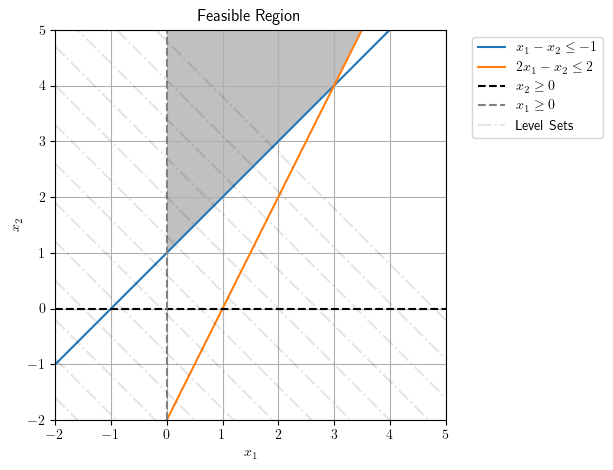
\includegraphics[width=0.7\textwidth]{problem_5_primal.png}
    \caption{Feasible region and level curves for the equivalent primal program.}
    \label{fig:problem_5_primal}
  \end{figure}

  \begin{mini*}
    {}{w = b^T y = -y'_1 + 2y_2}{}{}
    \addConstraint{ -y'_1 - 2y_2}{\le 1}
    \addConstraint{  y'_1 + y_2}{\le 1}
    \addConstraint{y'_1,}{y_2 \ge 0}.
  \end{mini*}

  We see in Figure \ref{fig:problem_5_dual} that the equivalent program is optimized at the point\linebreak
  $(y'_1, y_2)^T = (1, 0)^T$ (and $(y_1, y_2)^T = (-1, 0)^T$, by extension). The optimal solution for the dual is 
  thus given by $w = b^T y = y_1 + 2y_2 = -1 + 0 = z$ , as predicted by the strong duality theorem. 

  \begin{figure}[h]
    \centering
    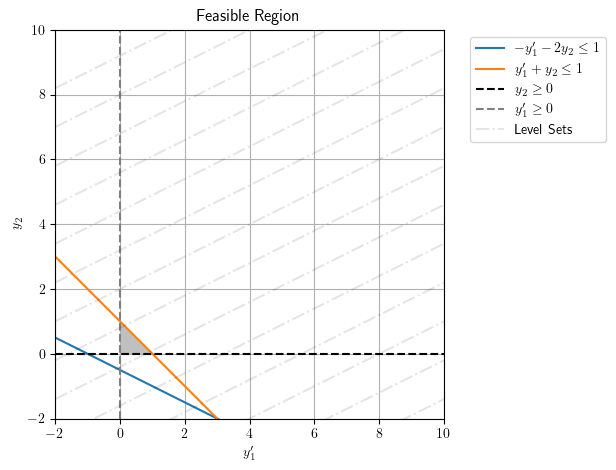
\includegraphics[width=0.7\textwidth]{problem_5_dual.png}
    \caption{Feasible region and level curves for the equivalent dual program.}
    \label{fig:problem_5_dual}
  \end{figure}

  To verify that the optimal dual solution satisfies $y^T = c_B^T B^{-1}$, we express the primal problem in standard 
  form and solve it using the two-phase simplex method. We introduce the excess variable $x_3$ and artificial variable 
  $x_4$ to the first constraint and slack variable $x_5$ to the second constraint. The primal problem in standard form 
  becomes:

  \begin{mini*}
    {}{\hat{z} = -z = x_1 + x_2}{}{}
    \addConstraint{-x_1 + x_2 - x_3 + x_4}{= 1}
    \addConstraint{2x_1 - x_2 + x_5}{= 2}
    \addConstraint{x_1, x_2}{\ge 0}.
  \end{mini*}

  With $x_B = (x_4, x_5)$ as our phase I feasible solution, we obtain the the initial basis
  $x_B = (x_2, x_4)^T$ for the phase II problem. This is coincidentally the optimal basic feasible solution for the
  second phase of the simplex method, and so we find\footnote{
    Details for these computations may be found by running \texttt{problem\_5.py}.
  }

  $$
  B = \begin{pmatrix}
        -1 & 0 \\
        -1 & 1
      \end{pmatrix}, \quad c_B^T = \begin{pmatrix*}
        1 \\
        0
      \end{pmatrix*}
  $$

  Hence we see
  
  \begin{align*}
    c_B^T B^{-1} &= \begin{pmatrix*} 1 & 0 \end{pmatrix*} \begin{pmatrix*}[r]
                      -1 & 0 \\
                      -1 & 1
                    \end{pmatrix*} \\
                 &= \begin{pmatrix*}
                      -1 & 0
                    \end{pmatrix*} \\
                 &= y^T 
  \end{align*}
        
  as desired.
  \ \\
\end{solution}
